\chapter{Implementation}
\label{implementation}

\section{Implementation}

\subsection{Psuedo Code}
Here is the psuedo code for traffic matrix generation with simple gravity model for Quantum Internet.

\begin{figure}[H]
  \begin{algorithm}[H]
    \caption{Traffic Matrix Generation with Simple Gravity Model for Quantum Internet}
    \label{alg1}
    \begin{algorithmic}
      \Require 
      $N$ (Number of nodes entire the network), \\
      $T^{initiator}(n_i) : i = 1, \cdots, N;$ (Number of sent requests) ,\\
      $T^{responder}(n_i) : i = 1, \cdots, N;$ (Number of received requests)
      \Ensure $T(n_i, n_k) : i = 1, \cdots, N; k = 1, \cdots, N$ (Traffic matrix)
      \For{$i=1,\cdots,N$}
        \State $T^{total}(n_k) \leftarrow 0$
        \For{$k=1,\cdots,N$}
          \If{$i \neq k$}
            \State $T^{total}(n_k) \leftarrow T^{total}(n_k) + T^{responder}(n_k)$
          \EndIf
        \EndFor
        \For{$k=1,\cdots,N$}
          \If{$i \neq k$}
            \State $T(n_i, n_k) \leftarrow T^{initiator}(n_i) \times (T^{responder}(n_k) / T^{total}(n_k))$
          \Else
            \State $T(n_i, n_k) \leftarrow 0$
          \EndIf
        \EndFor
      \EndFor
      \State \Return $T(n_i, n_k)$
    \end{algorithmic}
  \end{algorithm}
\end{figure}

According to the QuISP specification, each node has its own information about where it sent the setup request to.
Therefore, the implementation does not directly generate the traffic matrix for the network as a whole.
For this reason, in the gravity model, each node calculates the amount of traffic it sends from itself by retrieving data from other nodes. 
This is the specification in my implementation.

I implemented this in C++, the language of OMNeT++. 
You can see my actual code from code listings \ref{gravity_cpp}.

\subsection{Demo on QuISP}
\begin{figure}[H]
  \centering
  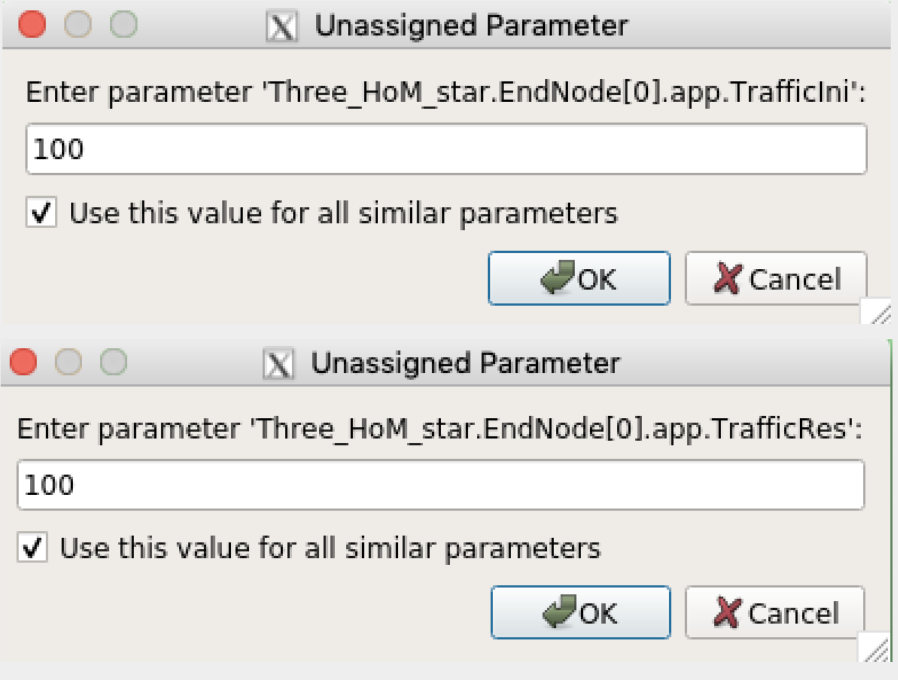
\includegraphics[width=10cm]{img/QuISP_input.png}
  \caption{Input Display in QuISP}
  \label{fig:QuISP_input} 
\end{figure}
When you set up the simulation, you will be asked for node data, as shown in the figure above.
You have to input the amount of initiator traffic and the amount of responder traffic for each node.
\begin{figure}[H]
  \centering
  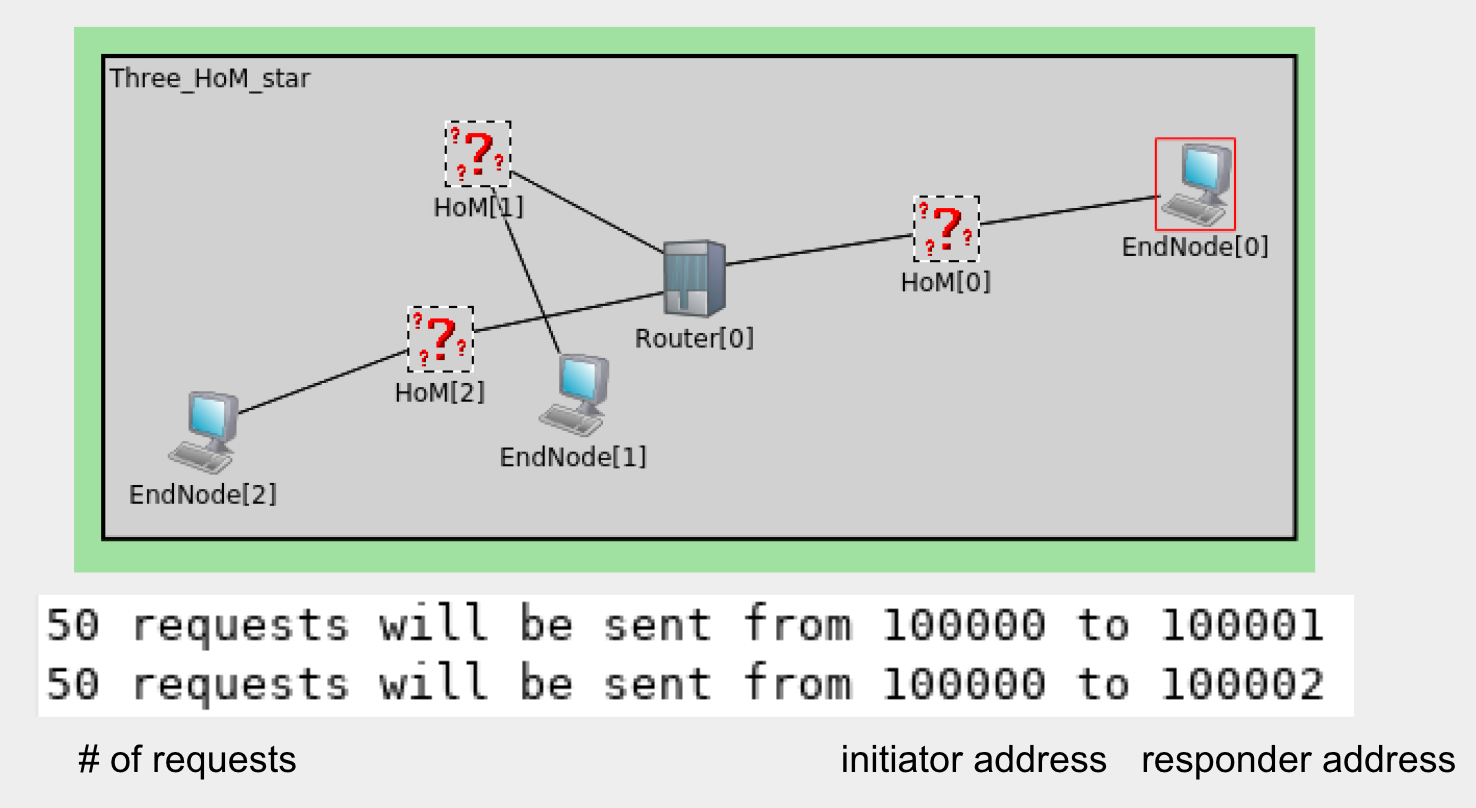
\includegraphics[width=10cm]{img/QuISP_result.png}
  \caption{Result Display in QuISP}
  \label{fig:QuISP_result} 
\end{figure}
After entering the node data and starting the simulation, the addresses of the initiator and responder and the amount of traffic between the two will be output.
%%% Local Variables:
%%% mode: japanese-latex
%%% TeX-master: "../bthesis"
%%% End: